\documentclass[a4paper, 11pt]{report}
\usepackage[utf8]{inputenc}
\usepackage{amsmath,tabto}
\usepackage{hyperref}
\usepackage{titlesec}
\usepackage{graphicx}
\graphicspath{ {images/} }

\usepackage{fullpage} % changes the margin
\usepackage{setspace}
\titleformat{\chapter}[display]
  {\normalfont\bfseries}{}{0pt}{\Large}
 \titlespacing*{\chapter}{0pt}{-50pt}{40pt}
\onehalfspacing
\date{}
\title{SOEN 6481 - System Software Requirements Specification
\newline Deliverable-1}

\author{
\normalsize  {Maria Ahmed}\\
\normalsize  {Adarsh Aravind}\\
\normalsize  {Sri Akhil Varma Alluri}\\
\normalsize  {Dheeraj Ashok Shobha}\\
\normalsize  {Charles Jebalitherson Augustin Moses}}
\begin{document}
\maketitle
 
\tableofcontents
\chapter{Problem 1}
\section{Introduction}
In this document, we will analyse and discuss(iGo) about the online ticket vending machine that can be used across all the cities of Canada. The requirements and use cases are recorded in the pictorial representation with the help of use modeling, problem domain modeling, stakeholders modeling and use case modeling for different perspectives.
\section{Scope}
The online ticket vending machine(iGo) is used to serve public transportation including buses and local trains(metro). iGo users will have an online platform to recharge their OPUS cards and manage all the transactions at one place. iGo does not have any scope for maintaining the existing physical TVM's in metro stations.
\section{Description of TVM (iGo)}
iGo is a online web application system where users can sign-up, login and recharge their OPUS cards. iGo will send all the data to STM's(Société de transport de Montréal) system through secured communication protocol. iGo involves variety of actors such as Government of Canada, Public Transport Authority(STM), Payment authority, customer, station master,.. which makes it an interesting domain to study. \\\\
The traveller must sign up an account with iGo for first time or they can sign in as guest user where transaction history will not be available. For signing up into the system, it is mandatory to enter OPUS card number. Only one OPUS card can be linked per user to avoid internal complexities and fraudulent use of OPUS card. Once the user is logged into the system, he/she can recharge their opus cards or purchase 1-way, 2-ways or weekend trip based on their requirement. New users can also see their transaction history at any point of time to better understand the usability of iGo.\\\\
iGo will provide following services to its users,

\begin{enumerate}
    \item A customer must be able to sign-up to an account online with their email address or mobile number or any social media account( Google, Facebook) and be able to link their OPUS card to personal iGo account.
    \item A customer must be able to make payment in one of three ways namely Master/ Visa debit card, Master/ Visa credit card and Paypal account. (If it's a web based application, why not interac?)
    \item A customer must be able to view their existing iGo wallet balance.
    \item A customer must be able to view their iGo transactions, and must be able to print out their transactions.
    \item A customer must be able to schedule the pre authorized payments for their OPUS cards.
    \item A customer must be able to add/ modify or delete personal information.
    \item A customer must be able to remove OPUS card from iGo account at any point of time.
    
\end{enumerate}

STM protects the customer information by handling the payments through high level secured communication protocol. iGo has in-built security feature  to validate the card, here iGo initiates a request to connect with financial institution. Once the connection is established, banking institution validates the given card against the PIN entered by the user. iGo has a strong established network that handles thousands of users on a daily basis and it is highly reliable.\\\\
iGo is also used to assist in management of queue and priority of services in financial institutions, universities, and customer help desks of several organizations. It saves the time, money and effort by providing the services in a quick and efficient manner. iGo is highly available but fails rarely due to power outage, internet service breakdown.\\\\
iGo will also maintain its internal log of transactions to resolve ambiguities arising from a connection failure in the middle of transaction between iGo and STM System. Al the events will be recorded in the log when a traveller registers an account, logs in and  also the web pages that user visits. This log data helps us to perform analytics and improve them to attract new customers.

\qquad\qquad\qquad\qquad 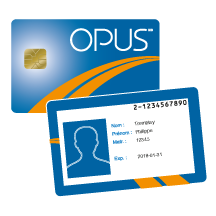
\includegraphics[width=70mm,scale=0.5]
{opus.png}\\
\tab\tab\qquad\qquad Fig.1 A Sample OPUS card (Source: Carte OPUS)


\end{document}
